\documentclass[spanish]{article}
\usepackage{titlesec}

%Quitar páginas en blanco
\let\cleardoublepage\clearpage
\usepackage{etoolbox}
\makeatletter
\patchcmd{\@endpart}{\vfil\newpage}{\par}{}{}
\makeatother

%\usepackage[spanish]{babel} ¡Esto estaba interfiriendo con las flechitas de los \tikspicture

\renewcommand{\contentsname}{Índice}

\usepackage[left=4cm, right=4cm]{geometry}
\usepackage{palatino}%Font
\usepackage{graphicx}
\usepackage{wrapfig}
\usepackage{float}
\usepackage{subcaption}
\usepackage{enumitem}
\usepackage{parskip}
\usepackage{multirow}
\usepackage{multicol}
\usepackage{booktabs}
\usepackage{amsthm}
\usepackage{amssymb}
\usepackage{amsmath}
\usepackage{cancel}
\usepackage{tikz}
\usepackage{tikz-cd}
\usepackage{tikz-3dplot}
\usepackage{xcolor}
\usepackage[bookmarks,bookmarksopen,bookmarksdepth=3]{hyperref}
\hypersetup{
	colorlinks=true,
	urlcolor=blue,
	linkcolor=magenta,
	citecolor=blue,
	filecolor=blue,
	urlbordercolor=white,
	linkbordercolor=white,
	citebordercolor=white,
	filebordercolor=white
}

\theoremstyle{definition}
\renewcommand{\proofname}{Demostración}

\newtheorem*{defn}{Definición}
\newtheorem*{lema}{Lema}
\newtheorem*{obs}{Observación}
\newtheorem*{teo}{Teorema}
\newtheorem*{prop}{Proposición}
\newtheorem*{coro}{Corolario}
\newtheorem*{af}{Afirmación}
\newtheorem*{ejer}{Ejercicio}
\newtheorem*{ejem}{Ejemplo}
\newtheorem*{pregunta}{Pregunta}
\newtheorem*{Wreg}{Construcción de Wythoff para poliedros regulares}
\newtheorem*{Wqui}{Construcción de Wythoff para poliedros quirales}

\newcommand{\R}{\mathbb{R}}
\newcommand{\Z}{\mathbb{Z}}
\newcommand{\N}{\mathbb{N}}
\newcommand{\C}{\mathbb{C}}
\newcommand{\Q}{\mathbb{Q}}
\newcommand{\s}{\mathbb{S}}
\newcommand{\PP}{\mathbb{P}}
\newcommand{\p}{\mathcal{P}}
\newcommand{\T}{\mathcal{T}}
\DeclareMathOperator{\img}{img}
\DeclareMathOperator{\Fix}{Fix}
\DeclareMathOperator{\Stab}{Stab}

%\definecolor{blue-violet}{rgb}{0.54, 0.17, 0.89}
\definecolor{azure}{rgb}{0.0, 0.5, 1.0}
\definecolor{green(ncs)}{rgb}{0.0, 0.62, 0.42}
\definecolor{forestgreen(web)}{rgb}{0.13, 0.55, 0.13}
\definecolor{limegreen}{rgb}{0.2, 0.8, 0.2}
\definecolor{palatinateblue}{rgb}{0.15, 0.23, 0.89}
\definecolor{trueblue}{rgb}{0.0, 0.45, 0.81}
\definecolor{goldenyellow}{rgb}{1.0, 0.87, 0.0}

\title{Un 4-politopo quiral a partir de un poliedro quiral}
\author{Tesina (borrador)\\Daniel González Casanova Azuela}
\date{}

\begin{document}
\maketitle
\begin{center}
	\large{\textbf{Resumen}}
\end{center}
En 2014, J. Bracho, I. Hubard y D. Pellicer encontraron un 4-politopo quiral en $\R^4$  \cite{bracho2013finite}. En este trabajo caracterizamos un nuevo 4-politopo quiral a partir de uno de los poliedros quirales construidos en \cite{bracho2021chiral}.

\phantomsection
\tableofcontents

\section{Introducción}
Este trabajo está situado en el contexto de los politopos altamente simétricos. Interesantemente, la definción de politopo ha cambiado mucho a través del tiempo. Siguiendo el trabajo de Grünbaum \cite{grunbaum1977regular}, desde hace algunas décadas se han estudiado los poliedros (y en general, politopos) "skeletal", cuyas caras no necesariamente son polígonos planos, y más bien se piensan como gráficas cíclicas en el conjunto de vértices.

Estudiamos estos politopos a través de la acción de su grupo de simetrías en los conjuntos de vértices, aristas, caras, etc. Un poliedro es regular cuando esta acción es transitiva en las banderas,que son ternas mutualmente incidentes de vértice, arista y cara. Un poliedro es quiral cuando esta acción induce dos órbitas en las banderas (y banderas adyacentes pertenecen a órbitas distintas), capturando la idea de tener máxima simetría rotacional pero sin reflexiones.

En 2014, J. Bracho, I. Hubard y D. Pellicer encontraron un 4-politopo quiral en $\R^4$, el cubo de Roli \cite{bracho2013chiral}. Las facetas (3-caras) de este politopo son poliedros quirales. En otro trabajo \cite{bracho2021finite}, los mismos autores desarrollaron un método para obtener un poliedro quiral a partir de un 4-politopo regular, entre los cuales está la faceta del cubo de Roli. En este trabajo construimos un 4-politopo quiral a partir de uno de los poliedros quirales en \cite{bracho2013chiral}.

\subsection{El cubo de Roli}
Mostramos una construcción informal de este cubo. Comenzamos con dos coloraciones de las aristas del 4-cubo. La coloración del lado izquierdo corresponde con la estructura usual del 4-cubo, mientras el del lado derecho tenemos el cubo de Roli. La diferencia entre ellos está en cómo definimos las caras y las facetas de cada uno; los vértices y las aristas son los mismos en ambos cubos. 

\tdplotsetmaincoords{70}{10} % Set the viewpoint angles (theta, phi)
\[\begin{tikzpicture}[scale=1.3, tdplot_main_coords, line width=2pt, line cap=round]
	% Define cube coordinates for the inner cube (smaller size)
	\coordinate (A) at (-0.5,-0.5,-0.5);
	\coordinate (B) at (-0.5,0.5,-0.5);
	\coordinate (C) at (0.5,0.5,-0.5);
	\coordinate (D) at (0.5,-0.5,-0.5);
	\coordinate (E) at (-0.5,-0.5,0.5);
	\coordinate (F) at (-0.5,0.5,0.5);
	\coordinate (G) at (0.5,0.5,0.5);
	\coordinate (H) at (0.5,-0.5,0.5);
	
	% Define cube coordinates for the outer cube (larger size)
	\coordinate (A2) at (-1.5,-1.5,-1.5);
	\coordinate (B2) at (-1.5,1.5,-1.5);
	\coordinate (C2) at (1.5,1.5,-1.5);
	\coordinate (D2) at (1.5,-1.5,-1.5);
	\coordinate (E2) at (-1.5,-1.5,1.5);
	\coordinate (F2) at (-1.5,1.5,1.5);
	\coordinate (G2) at (1.5,1.5,1.5);
	\coordinate (H2) at (1.5,-1.5,1.5);
	
	% Draw lines connecting the inner and outer cube vertices
	\draw[limegreen] (B2) -- (F2);%This one must be here
	\draw[blue] (B2) -- (C2);%And this one
	\draw[goldenyellow] (A) -- (A2);
	\draw[goldenyellow] (B) -- (B2);
	\draw[goldenyellow] (C) -- (C2);
	\draw[goldenyellow] (D) -- (D2);
	\draw[goldenyellow] (E) -- (E2);
	\draw[goldenyellow] (F) -- (F2);
	\draw[goldenyellow] (G) -- (G2);
	%\draw[limegreen] (H) -- (H2);
	
	% Draw inner cube edges
	%Y
	\draw[red] (C) -- (D);
	\draw[red] (A) -- (B);
	%\draw[red] (E) -- (F);
	%\draw[red] (G) -- (H);
	%Z
	\draw[limegreen] (A) -- (E);
	\draw[limegreen] (B) -- (F);
	\draw[limegreen] (C) -- (G);
	%\draw[blue-violet] (D) -- (H);
	%X
	\draw[blue] (B) -- (C);
	\draw[blue] (D) -- (A);
	\draw[blue] (F) -- (G);
	\draw[blue] (H) -- (E);
	\draw[limegreen] (D) -- (H);%This here
	\draw[red] (E) -- (F);%This ones here
	\draw[red] (G) -- (H);
	
	% Draw outer cube edges with random colors
	%Y
	\draw[red] (C2) -- (D2);
	\draw[red] (A2) -- (B2);
	\draw[red] (E2) -- (F2);
	\draw[red] (G2) -- (H2);
	%Z
	\draw[limegreen] (A2) -- (E2);
	%\draw[blue-violet] (B2) -- (F2);
	\draw[limegreen] (C2) -- (G2);
	\draw[goldenyellow] (H) -- (H2);%And this one here
	\draw[limegreen] (D2) -- (H2);
	%X
	%\draw[blue] (B2) -- (C2);
	\draw[blue] (D2) -- (A2);
	\draw[blue] (F2) -- (G2);
	\draw[blue] (H2) -- (E2);
\end{tikzpicture}\qquad\qquad\qquad\begin{tikzpicture}[scale=1.3, tdplot_main_coords, line width=2pt, line cap=round]
	% Define cube coordinates for the inner cube (smaller size)
	\coordinate (A) at (-0.5,-0.5,-0.5);
	\coordinate (B) at (-0.5,0.5,-0.5);
	\coordinate (C) at (0.5,0.5,-0.5);
	\coordinate (D) at (0.5,-0.5,-0.5);
	\coordinate (E) at (-0.5,-0.5,0.5);
	\coordinate (F) at (-0.5,0.5,0.5);
	\coordinate (G) at (0.5,0.5,0.5);
	\coordinate (H) at (0.5,-0.5,0.5);
	
	% Define cube coordinates for the outer cube (larger size)
	\coordinate (A2) at (-1.5,-1.5,-1.5);
	\coordinate (B2) at (-1.5,1.5,-1.5);
	\coordinate (C2) at (1.5,1.5,-1.5);
	\coordinate (D2) at (1.5,-1.5,-1.5);
	\coordinate (E2) at (-1.5,-1.5,1.5);
	\coordinate (F2) at (-1.5,1.5,1.5);
	\coordinate (G2) at (1.5,1.5,1.5);
	\coordinate (H2) at (1.5,-1.5,1.5);
	
	% Draw lines connecting the inner and outer cube vertices
	\draw[blue] (B2) -- (F2);%This one must be here
	\draw[limegreen] (B2) -- (C2);%And this one
	\draw[blue] (A) -- (A2);
	\draw[red] (B) -- (B2);
	\draw[goldenyellow] (C) -- (C2);
	\draw[limegreen] (D) -- (D2);
	\draw[goldenyellow] (E) -- (E2);
	\draw[limegreen] (F) -- (F2);
	\draw[blue] (G) -- (G2);
	%\draw[limegreen] (H) -- (H2);
	
	% Draw inner cube edges
	%Y
	\draw[red] (C) -- (D);
	\draw[limegreen] (A) -- (B);
	%\draw[red] (E) -- (F);
	%\draw[red] (G) -- (H);
	%Z
	\draw[red] (A) -- (E);
	\draw[goldenyellow] (B) -- (F);
	\draw[limegreen] (C) -- (G);
	%\draw[blue-violet] (D) -- (H);
	%X
	\draw[blue] (B) -- (C);
	\draw[goldenyellow] (D) -- (A);
	\draw[red] (F) -- (G);
	\draw[limegreen] (H) -- (E);
	\draw[blue] (D) -- (H);%This here
	\draw[blue] (E) -- (F);%This ones here
	\draw[goldenyellow] (G) -- (H);
	
	% Draw outer cube edges with random colors
	%Y
	\draw[blue] (C2) -- (D2);
	\draw[goldenyellow] (A2) -- (B2);
	\draw[red] (E2) -- (F2);
	\draw[limegreen] (G2) -- (H2);
	%Z
	\draw[limegreen] (A2) -- (E2);
	%\draw[blue-violet] (B2) -- (F2);
	\draw[red] (C2) -- (G2);
	\draw[red] (H) -- (H2);%And this one here
	\draw[goldenyellow] (D2) -- (H2);
	%X
	%\draw[blue] (B2) -- (C2);
	\draw[red] (D2) -- (A2);
	\draw[goldenyellow] (F2) -- (G2);
	\draw[blue] (H2) -- (E2);
\end{tikzpicture}\]
Notemos que las caras del 4-cubo usual son, en la coloración del lado izquierdo, los 4-ciclos de aristas de dos colores que van alternando. Definamos las caras del cubo de Roli como los 8-ciclos de aristas de dos colores que van alternando en la coloración del lado derecho. Aquí están las caras verde-rojo:
\[\begin{tikzpicture}[scale=1.3, tdplot_main_coords, line width=2pt, line cap=round]
	% Define cube coordinates for the inner cube (smaller size)
	\coordinate (A) at (-0.5,-0.5,-0.5);
	\coordinate (B) at (-0.5,0.5,-0.5);
	\coordinate (C) at (0.5,0.5,-0.5);
	\coordinate (D) at (0.5,-0.5,-0.5);
	\coordinate (E) at (-0.5,-0.5,0.5);
	\coordinate (F) at (-0.5,0.5,0.5);
	\coordinate (G) at (0.5,0.5,0.5);
	\coordinate (H) at (0.5,-0.5,0.5);
	
	% Define cube coordinates for the outer cube (larger size)
	\coordinate (A2) at (-1.5,-1.5,-1.5);
	\coordinate (B2) at (-1.5,1.5,-1.5);
	\coordinate (C2) at (1.5,1.5,-1.5);
	\coordinate (D2) at (1.5,-1.5,-1.5);
	\coordinate (E2) at (-1.5,-1.5,1.5);
	\coordinate (F2) at (-1.5,1.5,1.5);
	\coordinate (G2) at (1.5,1.5,1.5);
	\coordinate (H2) at (1.5,-1.5,1.5);
	
	% Draw lines connecting the inner and outer cube vertices
	\draw[limegreen] (B2) -- (F2);
	
	% Draw inner cube edges
	\draw[red] (C) -- (D);
	\draw[red] (A) -- (B);
	\draw[limegreen] (A) -- (E);
	\draw[limegreen] (B) -- (F);
	\draw[limegreen] (C) -- (G);
	\draw[limegreen] (D) -- (H);
	\draw[red] (E) -- (F);
	\draw[red] (G) -- (H);
	
	% Draw outer cube edges
	\draw[red] (C2) -- (D2);
	\draw[red] (A2) -- (B2);
	\draw[red] (E2) -- (F2);
	\draw[red] (G2) -- (H2);
	\draw[limegreen] (A2) -- (E2);
	\draw[limegreen] (C2) -- (G2);
	\draw[limegreen] (D2) -- (H2);
\end{tikzpicture}\qquad\qquad\qquad\begin{tikzpicture}[scale=1.3, tdplot_main_coords, line width=2pt, line cap=round]
	% Define cube coordinates for the inner cube (smaller size)
	\coordinate (A) at (-0.5,-0.5,-0.5);
	\coordinate (B) at (-0.5,0.5,-0.5);
	\coordinate (C) at (0.5,0.5,-0.5);
	\coordinate (D) at (0.5,-0.5,-0.5);
	\coordinate (E) at (-0.5,-0.5,0.5);
	\coordinate (F) at (-0.5,0.5,0.5);
	\coordinate (G) at (0.5,0.5,0.5);
	\coordinate (H) at (0.5,-0.5,0.5);
	
	% Define cube coordinates for the outer cube (larger size)
	\coordinate (A2) at (-1.5,-1.5,-1.5);
	\coordinate (B2) at (-1.5,1.5,-1.5);
	\coordinate (C2) at (1.5,1.5,-1.5);
	\coordinate (D2) at (1.5,-1.5,-1.5);
	\coordinate (E2) at (-1.5,-1.5,1.5);
	\coordinate (F2) at (-1.5,1.5,1.5);
	\coordinate (G2) at (1.5,1.5,1.5);
	\coordinate (H2) at (1.5,-1.5,1.5);
	
	% Draw lines connecting the inner and outer cube vertices
	\draw[limegreen] (B2) -- (C2);%And this one
	\draw[red] (B) -- (B2);
	\draw[limegreen] (D) -- (D2);
	\draw[limegreen] (F) -- (F2);
	%\draw[limegreen] (H) -- (H2);
	
	% Draw inner cube edges
	%Y
	\draw[red] (C) -- (D);
	\draw[limegreen] (A) -- (B);
	%\draw[red] (E) -- (F);
	%\draw[red] (G) -- (H);
	%Z
	\draw[red] (A) -- (E);
	\draw[limegreen] (C) -- (G);
	%\draw[blue-violet] (D) -- (H);
	%X
	\draw[red] (F) -- (G);
	\draw[limegreen] (H) -- (E);
	
	% Draw outer cube edges with random colors
	%Y
	\draw[red] (E2) -- (F2);
	\draw[limegreen] (G2) -- (H2);
	%Z
	\draw[limegreen] (A2) -- (E2);
	%\draw[blue-violet] (B2) -- (F2);
	\draw[red] (C2) -- (G2);
	\draw[red] (H) -- (H2);%And this one here
	%X
	%\draw[blue] (B2) -- (C2);
	\draw[red] (D2) -- (A2);
\end{tikzpicture}\]
De la misma manera, en ambos casos definamos las facetas como las componentes conexas de tres colores. Aquí están las facetas verde-rojo-azul:
\[\begin{tikzpicture}[scale=1.3, tdplot_main_coords, line width=2pt, line cap=round]
	% Define cube coordinates for the inner cube (smaller size)
	\coordinate (A) at (-0.5,-0.5,-0.5);
	\coordinate (B) at (-0.5,0.5,-0.5);
	\coordinate (C) at (0.5,0.5,-0.5);
	\coordinate (D) at (0.5,-0.5,-0.5);
	\coordinate (E) at (-0.5,-0.5,0.5);
	\coordinate (F) at (-0.5,0.5,0.5);
	\coordinate (G) at (0.5,0.5,0.5);
	\coordinate (H) at (0.5,-0.5,0.5);
	
	% Define cube coordinates for the outer cube (larger size)
	\coordinate (A2) at (-1.5,-1.5,-1.5);
	\coordinate (B2) at (-1.5,1.5,-1.5);
	\coordinate (C2) at (1.5,1.5,-1.5);
	\coordinate (D2) at (1.5,-1.5,-1.5);
	\coordinate (E2) at (-1.5,-1.5,1.5);
	\coordinate (F2) at (-1.5,1.5,1.5);
	\coordinate (G2) at (1.5,1.5,1.5);
	\coordinate (H2) at (1.5,-1.5,1.5);
	
	% Draw lines connecting the inner and outer cube vertices
	\draw[limegreen] (B2) -- (F2);%This one must be here
	\draw[blue] (B2) -- (C2);%And this one
	%\draw[limegreen] (H) -- (H2);
	
	% Draw inner cube edges
	%Y
	\draw[red] (C) -- (D);
	\draw[red] (A) -- (B);
	%\draw[red] (E) -- (F);
	%\draw[red] (G) -- (H);
	%Z
	\draw[limegreen] (A) -- (E);
	\draw[limegreen] (B) -- (F);
	\draw[limegreen] (C) -- (G);
	%\draw[blue-violet] (D) -- (H);
	%X
	\draw[blue] (B) -- (C);
	\draw[blue] (D) -- (A);
	\draw[blue] (F) -- (G);
	\draw[blue] (H) -- (E);
	\draw[limegreen] (D) -- (H);%This here
	\draw[red] (E) -- (F);%This ones here
	\draw[red] (G) -- (H);
	
	% Draw outer cube edges with random colors
	%Y
	\draw[red] (C2) -- (D2);
	\draw[red] (A2) -- (B2);
	\draw[red] (E2) -- (F2);
	\draw[red] (G2) -- (H2);
	%Z
	\draw[limegreen] (A2) -- (E2);
	%\draw[blue-violet] (B2) -- (F2);
	\draw[limegreen] (C2) -- (G2);
	\draw[limegreen] (D2) -- (H2);
	%X
	%\draw[blue] (B2) -- (C2);
	\draw[blue] (D2) -- (A2);
	\draw[blue] (F2) -- (G2);
	\draw[blue] (H2) -- (E2);
\end{tikzpicture}\qquad\qquad\qquad\begin{tikzpicture}[scale=1.3, tdplot_main_coords, line width=2pt, line cap=round]
	% Define cube coordinates for the inner cube (smaller size)
	\coordinate (A) at (-0.5,-0.5,-0.5);
	\coordinate (B) at (-0.5,0.5,-0.5);
	\coordinate (C) at (0.5,0.5,-0.5);
	\coordinate (D) at (0.5,-0.5,-0.5);
	\coordinate (E) at (-0.5,-0.5,0.5);
	\coordinate (F) at (-0.5,0.5,0.5);
	\coordinate (G) at (0.5,0.5,0.5);
	\coordinate (H) at (0.5,-0.5,0.5);
	
	% Define cube coordinates for the outer cube (larger size)
	\coordinate (A2) at (-1.5,-1.5,-1.5);
	\coordinate (B2) at (-1.5,1.5,-1.5);
	\coordinate (C2) at (1.5,1.5,-1.5);
	\coordinate (D2) at (1.5,-1.5,-1.5);
	\coordinate (E2) at (-1.5,-1.5,1.5);
	\coordinate (F2) at (-1.5,1.5,1.5);
	\coordinate (G2) at (1.5,1.5,1.5);
	\coordinate (H2) at (1.5,-1.5,1.5);
	
	% Draw lines connecting the inner and outer cube vertices
	\draw[blue] (B2) -- (F2);%This one must be here
	\draw[limegreen] (B2) -- (C2);%And this one
	\draw[blue] (A) -- (A2);
	\draw[red] (B) -- (B2);
	\draw[limegreen] (D) -- (D2);
	\draw[limegreen] (F) -- (F2);
	\draw[blue] (G) -- (G2);
	%\draw[limegreen] (H) -- (H2);
	
	% Draw inner cube edges
	%Y
	\draw[red] (C) -- (D);
	\draw[limegreen] (A) -- (B);
	%\draw[red] (E) -- (F);
	%\draw[red] (G) -- (H);
	%Z
	\draw[red] (A) -- (E);
	\draw[limegreen] (C) -- (G);
	%\draw[blue-violet] (D) -- (H);
	%X
	\draw[blue] (B) -- (C);
	\draw[red] (F) -- (G);
	\draw[limegreen] (H) -- (E);
	\draw[blue] (D) -- (H);%This here
	\draw[blue] (E) -- (F);%This ones here
	
	
	% Draw outer cube edges with random colors
	%Y
	\draw[blue] (C2) -- (D2);
	\draw[red] (E2) -- (F2);
	\draw[limegreen] (G2) -- (H2);
	%Z
	\draw[limegreen] (A2) -- (E2);
	%\draw[blue-violet] (B2) -- (F2);
	\draw[red] (C2) -- (G2);
	\draw[red] (H) -- (H2);%And this one here
	%X
	%\draw[blue] (B2) -- (C2);
	\draw[red] (D2) -- (A2);
	\draw[blue] (H2) -- (E2);
\end{tikzpicture}\]
El cubo de Roli es un 4-politopo quiral \cite{bracho2013finite}. Tiene la mitad de caras y la mitad de facetas de las que tiene el 4-cubo. Las facetas son poliedros quirales (combintorialmente regulares). En la siguiente sección mostraremos otros poliedros quirales, entre los cuales está la faceta del cubo de Roli.

\subsection{Poliedros quirales a partir de una construcción PC}
En esta sección analizamos \cite{bracho2021quiral}. Presentamos un método para obtener un poliedro quiral a partir de un 4-politopo regular. Esencialmente hay tres pasos:
\begin{enumerate}
	\item Calcular el poliedro de Petrie-Coxeter $PC_\alpha(\mathcal{T})$ para alguna $\alpha\in[0,1]$. Resulta ser regular o de clase $2_{\{0,2\}}$.
	\item Aplicar la halving operation para obtener $PC_\alpha(\mathcal{T})^\eta$.
	\item Aplicar la operación de 2-facetting (2-hole) para obtener $(PC_\alpha(\mathcal{T})^\eta)^\phi:=H_\alpha(\mathcal{T})$. Éste es un poliedro regular o quiral.
\end{enumerate}
Cuando comenzamos con el 4-cubo y tomamos $\alpha=0$ obtenemos la faceta del cubo de Roli.

\subsubsection{Definiciones}
\textbf{*Faltan*}
\begin{defn}Un poliedro $\p$ es
	\begin{itemize}
		\item \textbf{regular} (resp. \textbf{combinatoriamente regular}) si su grupo de simetrías $G(\p)$ (resp. grupo de automorfismos $\Gamma(\p))$ actúa transitivamente en las banderas.
		
		\item \textbf{quiral} (resp. \textbf{combinatoriamente quiral}) si $G(\p)$ (resp. $\Gamma(\p)$) induce dos órbitas en las banderas con la propiedad de que dos banderas adyacentes están en órbitas diferentes.
	\end{itemize}
\end{defn}
\begin{obs}
	Si $\p$ es regular o quiral, el grupo de simetrías actúa transitivamente en caras, aristas y vértices.
\end{obs}

\subsubsection{La construcción de Petrie-Coxeter}
Dado un 4-politopo regular $\T$, mostraremos cómo constuir un poliedro regular o quiral $PC(\T)$. Suponemos por el resto del texto que $\T$ tiene caras planas.

Se escoge número $\alpha$ entre 0 y 1. Para un vértice $v$ de $\T$ y una cara que contiene a $v$, definimos el punto $(v,c)_\alpha$ sobre el segmento que une $v$ con $c$ a distancia $d\alpha$ desde $v$, donde $d$ es la distancia entre ellos. Estos puntos serán los vértices del poliedro $PC_\alpha(\T)$.

Las aristas son (1) los segmentos que unen $(v,c)_\alpha$ con $(v',c)_\alpha$, donde $v$ y $v'$ son vértices en una misma arista de $\T$; y (2) los semgentos que unen  $(v,c)_\alpha$ con $(v,c')_\alpha$ donde $c$ y $c'$ son facetas que comparten una cara conde está $v$.

Las caras son los cuadrados $(v,c)_\alpha$, $(v',c)_\alpha$, $(v,c')_\alpha$ y $(v',c')_\alpha$ donde $c$ y $c'$ son caras que contienen a la arista entre $v$ y $v'$.

\begin{figure}[H]
	\centering
	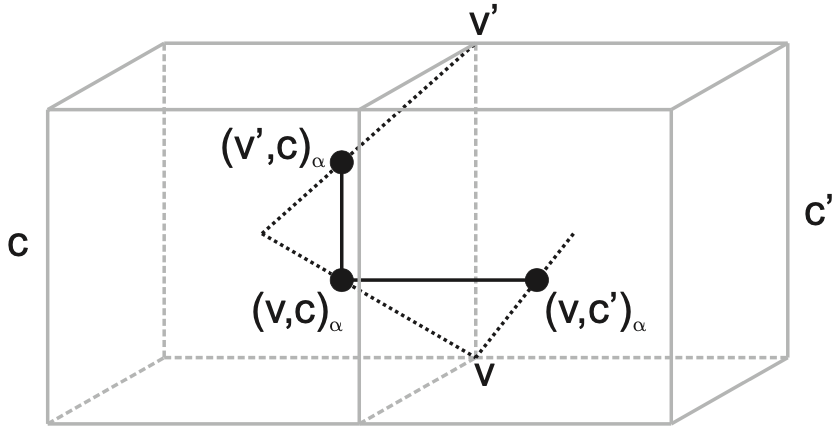
\includegraphics[width=0.5\linewidth]{p3}
	\caption*{Imagen de \cite{bracho2021quiral}}
\end{figure}
Tenemos algunos resultados sobre esta construcción:
\begin{teo}
	Para cualquier $\alpha\in(0,1)$ y cualquier politopo regular $\T$, $PC_\alpha(\T)$ es un poliedro.
\end{teo}
\begin{obs}
	Para cualesquiera $\alpha\in(0,1)$, un 4-politopo regular $\T$ y su dual $\T^*$, $PC_\alpha(\T)=PC_{1-\alpha}(\T)$.
\end{obs}
\begin{teo}
	Para cualesquiera $\alpha\in(0,1)$, un 4-politopo regular $\T$, el grupo de simetría de $\T$ es isomorfo a un subgrupo de índice a lo más 2 de $G(PC_\alpha(\T))$. Además, $PC_\alpha(\T)$ es regular o un poliedro de dos órbitas en la clase $2_{\{0,2\}}$.
\end{teo}
%\begin{figure}[H]
%	\centering
%	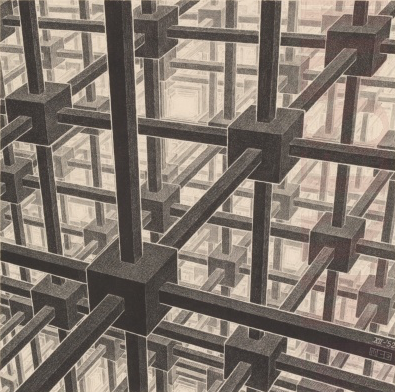
\includegraphics[width=0.45\linewidth]{p2}
%	\caption*{La construcción de Petrie-Coxeter y los valores de $\alpha$.}
%\end{figure}
\subsubsection{Halving operation}
\tdplotsetmaincoords{70}{15} % Set the viewpoint angles (theta, phi)
\[\begin{tikzpicture}[scale=3, tdplot_main_coords, line width=2pt, line cap=round]
	% Define cube coordinates for the inner cube (smaller size)
	\coordinate (A) at (-0.5,-0.5,-0.5);
	\coordinate (B) at (-0.5,0.5,-0.5);
	\coordinate (C) at (0.5,0.5,-0.5);
	\coordinate (D) at (0.5,-0.5,-0.5);
	\coordinate (E) at (-0.5,-0.5,0.5);
	\coordinate (F) at (-0.5,0.5,0.5);
	\coordinate (G) at (0.5,0.5,0.5);
	\coordinate (H) at (0.5,-0.5,0.5);
	
	% Draw inner cube edges
	\draw[limegreen] (C) -- (D);
	\draw[limegreen] (A) -- (B);
	\draw[limegreen] (A) -- (E);
	\draw[limegreen] (B) -- (F);
	\draw[limegreen] (C) -- (G);
	\draw[limegreen] (B) -- (C);
	\draw[limegreen] (D) -- (A);
	\draw[limegreen] (F) -- (G);
	\draw[limegreen] (H) -- (E);
	\draw[limegreen] (D) -- (H);
	\draw[limegreen] (E) -- (F);
	\draw[limegreen] (G) -- (H);
	
	\draw[blue] (A) -- (H);
	\draw[blue] (F) -- (H);
	\draw[blue] (F) -- (A);
	\draw[blue] (C) -- (H);
	\draw[blue] (A) -- (C);
	\draw[blue] (F) -- (C);
\end{tikzpicture}\]
Esta operación transforma un poliedro $\p$ con caras cuadradas en otro poliedro $\p^\eta$, cuyos vértices son algunos de los vértices de $\p$, donde dos de ellos son adyacentes si y sólo si son vértices opuestos en una cara de $\p$. Las caras de $\p^\eta$ con figuras de vértice de algunos de los vértices de $\p$.

Como $PC_\alpha(\T)$ tiene caras cuadradas, le podemos aplicar esta operación. Y como además es regular o de clase $2_{\{0,2\}}$, cualquier de los resultados de aplicarle la operación Halving son isomorfos.


\subsubsection{2-Hole}
A 2-hole is constructed by traversing an edge to one of its endpoints, skipping the first edge on the left according to some local orientation, and then traversing a second edge. This procedure is repeated until an edge is traversed twice in the same direction.

La operación Facetting o 2-Hole convierte un poliedro $\p$ con vértices de grado al menos 5 en una estructura $\p^\phi$ cuyo 1-esqueleto está contenido en el 1-esqueleto de $\p$ y sus caras son un subconjunto de los 2-hoyos de $\p$.

Dados un vértice, arista y un 2-hoyo incidentes, se va construyendo $\p^\phi$ por pasos de forma que el 1-esqueleto sea conexo y cada arista pertenezca a exactamente dos 2-hoyos. El resultado no siempre es un poliedro, pero en nuestro caso sí lo es. Esto es consecuencia del siguiente resultado:

\begin{teo}
	Cuando $PC_\alpha(\T)^\eta$ es un poliedro, es regular o de clase $2_{\{1\}}$.
\end{teo}

\begin{figure}[H]
	\centering
	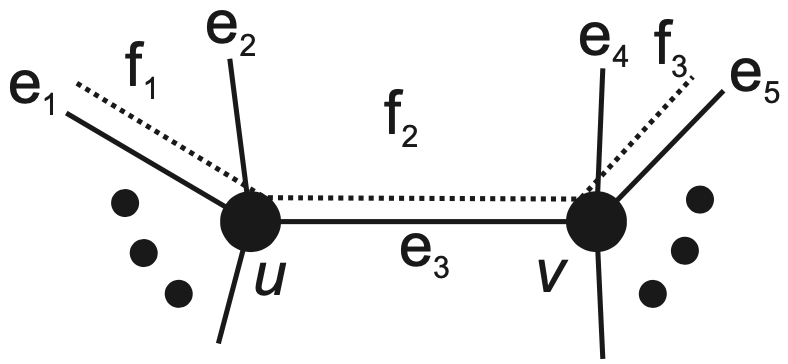
\includegraphics[width=0.5\linewidth]{p4}
	\caption*{Construcción de un 2-hoyo}
\end{figure}

\subsubsection{Poliedros quirales}
Finalmente podemos definir
\[H_\alpha(\T)=\left(PC_\alpha(\T)^\eta\right)^\phi\]
Para entender cómo construir los grupos de simetrías de estos poliedros, debemos recordar algunas cosas. Dado un poliedro $\p$ regular o quiral, el subgrupo de automorfismos $\Gamma^+(\p)$ está generado por dos rotaciones distinguidas: la de la cara, $\sigma_1$ y la del vértice $\sigma_2$.

Cuando $\p$ es plano (todas sus caras están en un plano, por ejemplo, el hemicubo en $\PP^2$), es posible que haya más de una isometría que actúa como $\sigma_1$ y $\sigma_2$.  Sin embargo, si $\p$ no es plano, son únicas.:
\begin{teo}
	Si $\p$ es un poliedro regular o quiral con caras planas, existen únicas isometrías $S_1$ y $S_2$ que actúan como $\sigma_1$ y $\sigma_2$ con respecto a alguna bandera base $\Phi$.
\end{teo}
Y luego,
\begin{prop}
	Si $H_\alpha(\T)$ es un poliedro, es regular o quiral.
\end{prop}
%\begin{proof}
%	Basta mostrar que existe la rotación de la cara $S_1$ y la rotación del vértice $S_2$. ¿Por qué? Si el grupo de simetrías del poliedro está generado por estas dos simetrías, queremos deducir que hay una o dos órbitas en banderas.
%\end{proof}

Se hizo este procedimiento para cada uno de los 4-politopos regulares (6 convexos y 10 estrellados). Veamos cómo analizar los poliedros resultantes.

De la regularidad de $\mathcal{T}$ podemos estudiar la simetría de $H_\alpha(\mathcal{T})$. Mientras que $G(\mathcal{T})=\langle R_0,R_1,R_2,R_3\rangle$ como en la construcción Wythoff, resulta que $G(H_\alpha(\mathcal{T}))\leq \langle S_1,S_2\rangle$, donde
\begin{align*}
	S_1&=R_0R_1R_3R_2\\
	S_2&=R_2R_1
\end{align*}
Aquí, $S_1$ es un tornillo y $S_2$ una rotación, dando lugar a la notación $\left\{\frac{p}{p_1,p_2},q\right\}$ donde $q$ es el orden de la rotación y los enteros $p,p_1$ y $p_2$ caracterizan al tornillo. Esto sugiere qué clase de poliedro es $H_\alpha(\mathcal{T})$: tiene caras helicoidales, $q$ en cada vértice.

Se encontraron los siguientes \textbf{Quiralitos} o \textbf{Halving-2-Holes}:

\begin{center}
	\begin{tabular}{|c|c|c|c|c|c|}
		\hline
		&\multirow{2}{*}{4-politopo} &\multirow{2}{*}{Quiralito}&  \multirow{3}{*}{$\#(G)$} &\multirow{3}{*}{$[G:\Gamma^+]$}& Colapsa\\
		&\multirow{2}{*}{ $\T$}&\multirow{2}{*}{$H_\alpha(T)$}&&&cuando\\
		&&&&&$\alpha=(0,1)$ \\
		\hline\hline
		\multirow{5}{*}{\rotatebox{90}{Convexos}}&\{3,3,3\} & $\{\frac{5}{1,2},3\}$ &60& 1 & (4,4) \\
		&\{4,3,3\} & $\{\frac{8}{1,3},3\}$ &48& 4&(1,2) \\
		&\{3,4,3\} & $\{\frac{12}{1,5},4\}$ &192&3&(2,2) \\
		&\{5,3,3\} & $\{\frac{30}{1,11},3\}$ &1440&5&(1,4)\\
		\hline
		\multirow{6}{*}{\rotatebox{90}{Estrellados}}&\{3,5,5/2\} &$\{\frac{20}{1,9},5\}$&1200&6&(2,2)\\
		&\{5,5/2,5\} & $\{\frac{15}{1,4},5/2\}$ &7200&1&(12,12)\\\cline{2-6}
		&\textcolor{magenta}{\{5,3,5/2\}} & $\{\frac{12}{1,5},3\}$ &144&50&(1,1)\\\cline{2-6}
		&\textcolor{magenta}{\{3,3,5/2\}}&$\{\frac{30}{7,13},3\}$& 1440 & 5 &(4,1)\\\cline{2-6}
		&\{3,5/2,5\}& $\{\frac{20}{3,7},5/2\}$ &1200&6& (2,2) \\
		&\{5/2,5,5/2\} & $\{\frac{15}{2,7},5\}$ &7200&1& (12,12)\\
		\hline
	\end{tabular}
\end{center}
Donde $G$ es el grupo de simetrías del quiralito.

Distintos valores de $\alpha$ en la construcción de Petrie-Coxeter dan lugar a distintos poliedros. Hay ciertos valores para los cuales las simetrías que generan $H_\alpha(\mathcal{T})$ son simetrías de $\mathcal{T}$. Cuando $\alpha=0$, los vértices de $PC_\alpha(\mathcal{P})$ son los vértices de $\mathcal{P}$.

Cuando $\alpha=0,1$, es posible que algunos de los vértices en la construcción "colapsen". Eso quiere decir que algunos vértices terminan siendo el mismo, y el resultado puede no ser un poliedro. Si, en cambio, aparece el valor 1, leemos que "la cantidad de vértices que colapsan es 1" (para $\alpha=0$ si el 1 está a la izquierda, y respectivamente $\alpha=1$ derecha). Es decir, no hay colapso.

Conviene entonces estudiar los casos donde no hay colapso para $\alpha=0$ pues en este caso la construcción de Petrie-Coxeter nos devuelve una estructura cuyos vértices son los mismos vértices del 4-politopo. Así, podremos usar las simetrías del 4-politopo original.

\section{Construcción de un 4-politopo quiral}
Aquí comienza nuestro trabajo, basado en la siguiente sospecha: así como el cubo de Roli es la faceta de un 4-politopo quiral, 

\begin{quote}\textbf{hay tres de los quiralitos que son las facetas de ciertos 4-politopos quirales.}\end{quote}

Los sospechosos son $H_1\{5,3,5/2\}$, $H_0\{5,3,5/2\}$ y $H_1\{3,3,5/2\}$. Se trata de los quiralitos obtenidos a partir de los 4-politopos estrellados "Gran 120-celda" y "Gran 600-celda", resp. Dos de ellos están escogidos para valores de $\alpha=1$, de forma que en estos dos casos estaremos trabajando con los 4-politopos duales, el \{5/2,5,3\} "Pequeño 120-celda estelado" y el \{5/2,3,3\}, "Gran gran 120-celda estelada". \textcolor{magenta}{\textbf{¡Hasta ahora hemos trabajado sólo con uno de estos tres! Es posible que se logre incluir un segundo en este mismo trabajo.}}

El primer paso es obtener los grupos de los 4-politopos regulares.

\subsection{Grupo de simetrías del \{5/2,3,5\}}
Comenzamos con el grupo del \{5/2,3,5\}. El grupo se denota [5/2,3,5]. La idea es tomar el grupo de simetrías de alguno de los convexos y expresar las relaciones del estrellado en términos de aquéllas.

\begin{figure}[H]
	\centering
	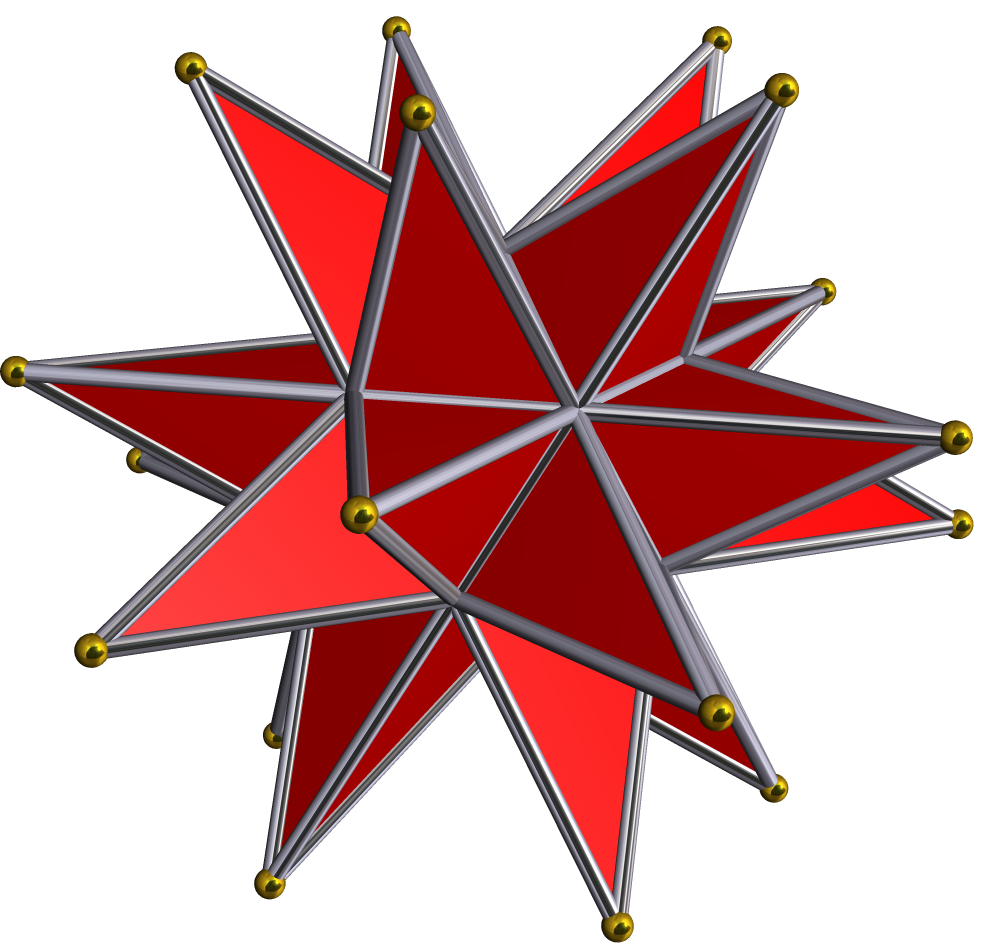
\includegraphics[width=0.4\linewidth]{p9}
	\caption*{\small{Las facetas del \{5/2,3,5\} son \{5/2,3\}, un tipo de poliedro estrellado regular (img:Wikipedia)}}
\end{figure}


En nuestro caso, partimos de que el grupo de la 600-celda, [3,3,5], está generado por $R_0,R_1,R_2$ y $R_3$. El objetivo es expresar expresar los generadores $P_0,P_1,P_2$ y $P_3$ del grupo [5/2,3,5] en términos de las $R_i$.

Recordemos que estos dos grupos tienen las siguientes presentaciones:
\begin{align*}\label{rels}
	[3,3,5]=&\langle R_i|R_i^2=(R_0R_1)^3=(R_1R_2)^3=(R_2R_3)^5=1\\
	&\qquad\qquad(R_0R_2)^2=(R_0R_3)^2=(R_1R_3)^2=1\rangle\\ \\
	[5/2,3,5]=&\langle P_i|P_i^2=(P_0P_1)^5=(P_1P_2)^3=(P_2P_3)^5=1\\
	&\qquad\qquad(P_0P_2)^2=(P_0P_3)^2=(P_1P_3)^2=1\rangle
\end{align*}
Los vértices falsos del \{5/2,3\}, que se forman en las intersecciones de las aristas pero no son vértices del poliedro, forman un icosaedro. La figura de vértice del \{3,3,5\} también es un icosaedro, respecto al cual podemos situar isometrías $R_i$.
\begin{af} Al hacer actuar el grupo [3,3,5] sobre el \{5/2,3\} de esta forma recostruimos el \{5/2,3,5\}.
\end{af}
\begin{proof}
	Basta dar una presentación del [5/2,3,5] como arriba. Definamos 
	\[P_0=R_0,\qquad P_2=R_3,\qquad P_3=R_2\]
	Para $P_1$ hay que hacer más trabajo.
	
	Mostramos dibujos \textit{aproximados} para desarrollar intuición (los objetos realmente están en dimensión 4). El tetraedro que vemos es una faceta del \{3,3,5\} pensada en el icosaedro de los vértices falsos del \{5/2,3\}. La conjugación $R_2R_3R_2$ es reflejar respecto a la cara de "en frente":
	\begin{figure}[H]
		\begin{subfigure}{0.4\linewidth}
			\centering
			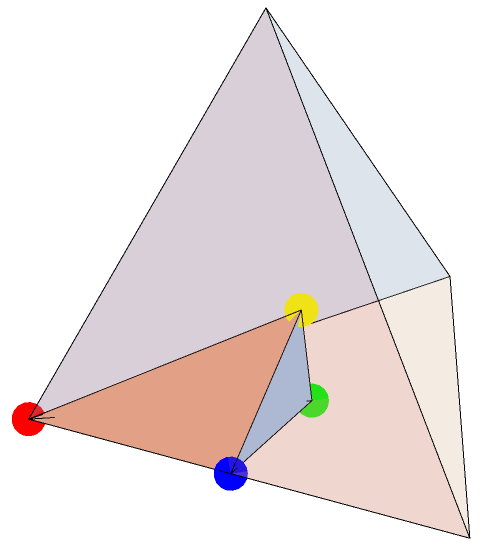
\includegraphics[width=0.6\linewidth]{p5}
		\end{subfigure}
		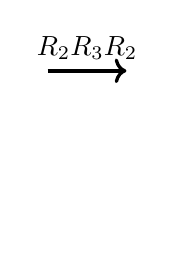
\begin{tikzpicture}
			\draw[->,very thick] (0,0)--(1,0) node[midway, above] {$R_2R_3R_2$};;
			\filldraw[white] (0,-2) circle (0.05);
		\end{tikzpicture}
		\begin{subfigure}{0.5\linewidth}
			\centering
			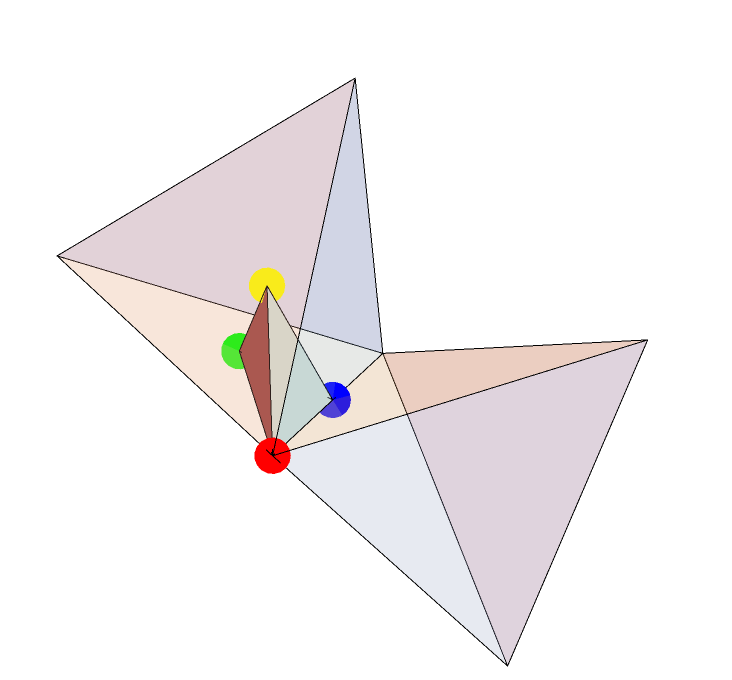
\includegraphics[width=0.9\linewidth]{p6}
		\end{subfigure}
	\end{figure}
	Ahora rotemos respecto a la recta amarillo-verde en dirección antihoraria (vista desde arriba), $R_0R_1$:
	\begin{figure}[H]
		\begin{subfigure}{0.4\linewidth}
			\centering
			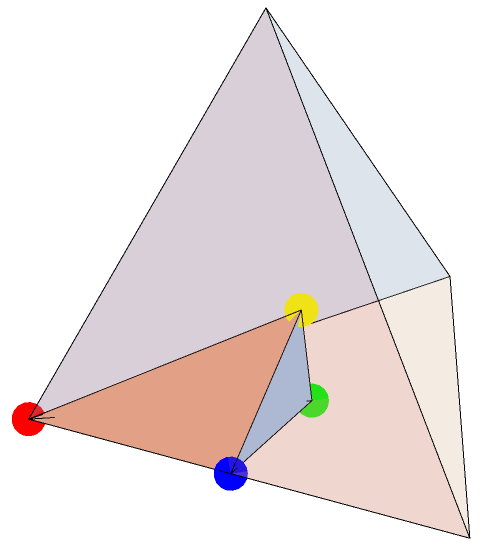
\includegraphics[width=0.6\linewidth]{p5}
		\end{subfigure}
		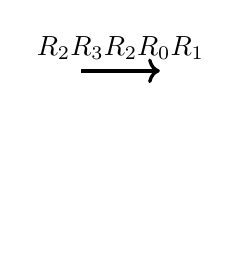
\begin{tikzpicture}
			\draw[->,very thick] (0,0)--(1,0) node[midway, above] {$R_2R_3R_2R_0R_1$};;
			\filldraw[white] (0,-2) circle (0.05);
		\end{tikzpicture}
		\begin{subfigure}{0.4\linewidth}
			\centering
			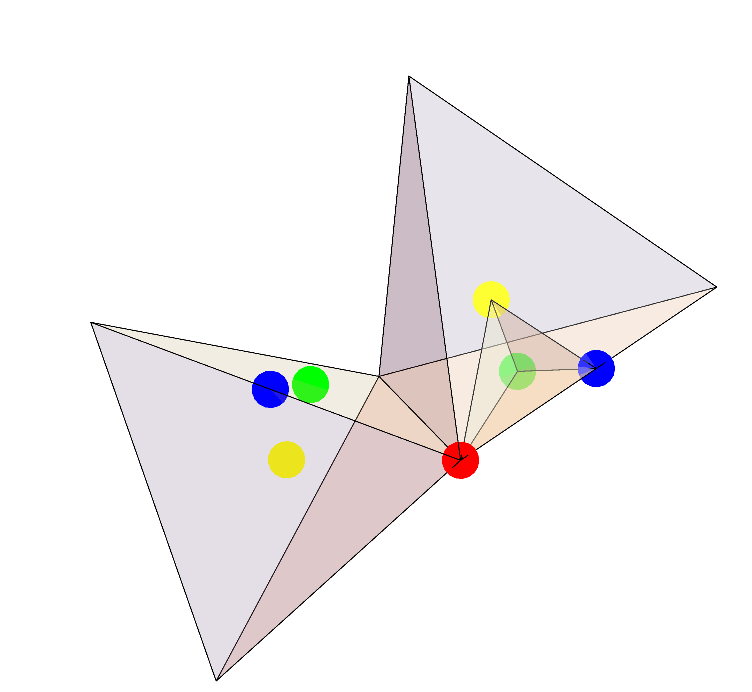
\includegraphics[width=0.9\linewidth]{p7}
		\end{subfigure}
	\end{figure}
	La observación clave es que la reflexión que buscamos está dada por el plano al que acaban de ir a dar los puntos rojo, verde y amarillo, de manera que $P_1$ es el conjugado de $R_1$ por la transformación que tenemos arriba.
	\begin{align*}
		P_1:=&(R_2R_3R_2R_0R_1)^{-1}R_1(R_2R_3R_2R_0R_1)\\
		=&R_1R_0R_2R_3R_2R_1R_2R_3R_2R_0R_1\\
		=&R_1R_2R_3R_2R_1R_0R_1R_2R_3R_2R_1
	\end{align*}
	Ahora veamos que se satisfacen las relaciones. Primero las que no tienen a $P_1$:
	\[(P_0P_2)^2=(R_0R_3)^2=1\qquad (P_0P_3)^2=(R_0R_2)^2=1\qquad (P_2P_3)^5=(R_3R_2)^5=1\]
	Dos de las relaciones faltantes se pueden consultar en el apéndice, y la última fue confirmada en GAP.
\end{proof}

\section{Construcción del 4-politopo quiral}
En \cite{bracho2021chiral} tenemos las siguientes fórmulas para construir un poliedro quiral dadas las simetrías que generan el grupo del 4-politopo regular:
\begin{align*}
	S_1&=P_0P_1P_3P_2\\
	S_2&=P_2P_1
\end{align*}
El resultado central de la tesina es proponer una tercera simetría $S_3$ mediante la cual se genere un 4-politopo quiral.

Analicemos el caso del Cubo de Roli para encontrar motivación. Escojamos una arista base, color azul clarito. ¿Qué debería hacer $S_3$? Bueno, simplemente debe girar el 4-politopo alrededor de la arista. Esto es justo lo que vemos en las tres figuras de abajo.
\begin{figure}[H]
	\begin{subfigure}{0.5\textwidth}
		\begin{tikzpicture}[scale=1.3, tdplot_main_coords, line width=2pt, line cap=round]
			\coordinate (A) at (-0.5,-0.5,-0.5);
			\coordinate (B) at (-0.5,0.5,-0.5);
			\coordinate (C) at (0.5,0.5,-0.5);
			\coordinate (D) at (0.5,-0.5,-0.5);
			\coordinate (E) at (-0.5,-0.5,0.5);
			\coordinate (F) at (-0.5,0.5,0.5);
			\coordinate (G) at (0.5,0.5,0.5);
			\coordinate (H) at (0.5,-0.5,0.5);
			
			% Define cube coordinates for the outer cube (larger size)
			\coordinate (A2) at (-1.5,-1.5,-1.5);
			\coordinate (B2) at (-1.5,1.5,-1.5);
			\coordinate (C2) at (1.5,1.5,-1.5);
			\coordinate (D2) at (1.5,-1.5,-1.5);
			\coordinate (E2) at (-1.5,-1.5,1.5);
			\coordinate (F2) at (-1.5,1.5,1.5);
			\coordinate (G2) at (1.5,1.5,1.5);
			\coordinate (H2) at (1.5,-1.5,1.5);
			
			% Draw lines connecting the inner and outer cube vertices
			\draw[limegreen] (B2) -- (F2);%This one must be here
			\draw[blue] (B2) -- (C2);%And this one
			\draw[goldenyellow] (A) -- (A2);
			\draw[goldenyellow] (B) -- (B2);
			\draw[goldenyellow] (C) -- (C2);
			\draw[goldenyellow] (D) -- (D2);
			\draw[goldenyellow] (E) -- (E2);
			\draw[goldenyellow] (F) -- (F2);
			\draw[goldenyellow] (G) -- (G2);
			%\draw[limegreen] (H) -- (H2);
			
			% Draw inner cube edges
			%Y
			\draw[red] (C) -- (D);
			\draw[red] (A) -- (B);
			%\draw[red] (E) -- (F);
			%\draw[red] (G) -- (H);
			%Z
			\draw[limegreen] (A) -- (E);
			\draw[limegreen] (B) -- (F);
			\draw[limegreen] (C) -- (G);
			%\draw[blue-violet] (D) -- (H);
			%X
			\draw[blue] (B) -- (C);
			\draw[blue] (D) -- (A);
			\draw[blue] (F) -- (G);
			\draw[blue] (H) -- (E);
			\draw[limegreen] (D) -- (H);%This here
			\draw[red] (E) -- (F);%This ones here
			\draw[red] (G) -- (H);
			
			% Draw outer cube edges with random colors
			%Y
			\draw[red] (C2) -- (D2);
			\draw[red] (A2) -- (B2);
			\draw[red] (E2) -- (F2);
			\draw[red] (G2) -- (H2);
			%Z
			\draw[limegreen] (A2) -- (E2);
			%\draw[blue-violet] (B2) -- (F2);
			\draw[limegreen] (C2) -- (G2);
			\draw[goldenyellow] (H) -- (H2);%And this one here
			\draw[limegreen] (D2) -- (H2);
			%X
			%\draw[blue] (B2) -- (C2);
			\draw[blue] (D2) -- (A2);
			\draw[blue] (F2) -- (G2);
			\draw[blue] (H2) -- (E2);
		\end{tikzpicture}
		\caption*{4-cubo}
	\end{subfigure}
	\begin{subfigure}{0.5\textwidth}
		\begin{tikzpicture}[scale=1.3, tdplot_main_coords, line width=2pt, line cap=round]
			% Define cube coordinates for the inner cube (smaller size)
			\coordinate (A) at (-0.5,-0.5,-0.5);
			\coordinate (B) at (-0.5,0.5,-0.5);
			\coordinate (C) at (0.5,0.5,-0.5);
			\coordinate (D) at (0.5,-0.5,-0.5);
			\coordinate (E) at (-0.5,-0.5,0.5);
			\coordinate (F) at (-0.5,0.5,0.5);
			\coordinate (G) at (0.5,0.5,0.5);
			\coordinate (H) at (0.5,-0.5,0.5);
			
			% Define cube coordinates for the outer cube (larger size)
			\coordinate (A2) at (-1.5,-1.5,-1.5);
			\coordinate (B2) at (-1.5,1.5,-1.5);
			\coordinate (C2) at (1.5,1.5,-1.5);
			\coordinate (D2) at (1.5,-1.5,-1.5);
			\coordinate (E2) at (-1.5,-1.5,1.5);
			\coordinate (F2) at (-1.5,1.5,1.5);
			\coordinate (G2) at (1.5,1.5,1.5);
			\coordinate (H2) at (1.5,-1.5,1.5);
			
			% Draw lines connecting the inner and outer cube vertices
			\draw[blue] (B2) -- (F2);%This one must be here
			\draw[limegreen] (B2) -- (C2);%And this one
			\draw[blue] (A) -- (A2);
			\draw[red] (B) -- (B2);
			\draw[goldenyellow] (C) -- (C2);
			\draw[limegreen] (D) -- (D2);
			\draw[goldenyellow] (E) -- (E2);
			\draw[limegreen] (F) -- (F2);
			\draw[blue] (G) -- (G2);
			%\draw[limegreen] (H) -- (H2);
			
			% Draw inner cube edges
			%Y
			\draw[red] (C) -- (D);
			\draw[limegreen] (A) -- (B);
			%\draw[red] (E) -- (F);
			%\draw[red] (G) -- (H);
			%Z
			\draw[red] (A) -- (E);
			\draw[goldenyellow] (B) -- (F);
			\draw[limegreen] (C) -- (G);
			%\draw[blue-violet] (D) -- (H);
			%X
			\draw[blue] (B) -- (C);
			\draw[goldenyellow] (D) -- (A);
			\draw[red] (F) -- (G);
			\draw[cyan] (H) -- (E);
			\draw[blue] (D) -- (H);%This here
			\draw[blue] (E) -- (F);%This ones here
			\draw[goldenyellow] (G) -- (H);
			
			% Draw outer cube edges with random colors
			%Y
			\draw[blue] (C2) -- (D2);
			\draw[goldenyellow] (A2) -- (B2);
			\draw[red] (E2) -- (F2);
			\draw[limegreen] (G2) -- (H2);
			%Z
			\draw[limegreen] (A2) -- (E2);
			%\draw[blue-violet] (B2) -- (F2);
			\draw[red] (C2) -- (G2);
			\draw[red] (H) -- (H2);%And this one here
			\draw[goldenyellow] (D2) -- (H2);
			%X
			%\draw[blue] (B2) -- (C2);
			\draw[red] (D2) -- (A2);
			\draw[goldenyellow] (F2) -- (G2);
			\draw[blue] (H2) -- (E2);
		\end{tikzpicture}
		\caption*{Cubo de Roli}
	\end{subfigure}
\end{figure}
\hspace{-1.3cm}
\begin{figure}[H]
	\begin{subfigure}{0.3\textwidth}
		\begin{tikzpicture}[scale=1, tdplot_main_coords, line width=2pt, line cap=round]
			% Define cube coordinates for the inner cube (smaller size)
			\coordinate (A) at (-0.5,-0.5,-0.5);
			\coordinate (B) at (-0.5,0.5,-0.5);
			\coordinate (C) at (0.5,0.5,-0.5);
			\coordinate (D) at (0.5,-0.5,-0.5);
			\coordinate (E) at (-0.5,-0.5,0.5);
			\coordinate (F) at (-0.5,0.5,0.5);
			\coordinate (G) at (0.5,0.5,0.5);
			\coordinate (H) at (0.5,-0.5,0.5);
			
			% Define cube coordinates for the outer cube (larger size)
			\coordinate (A2) at (-1.5,-1.5,-1.5);
			\coordinate (B2) at (-1.5,1.5,-1.5);
			\coordinate (C2) at (1.5,1.5,-1.5);
			\coordinate (D2) at (1.5,-1.5,-1.5);
			\coordinate (E2) at (-1.5,-1.5,1.5);
			\coordinate (F2) at (-1.5,1.5,1.5);
			\coordinate (G2) at (1.5,1.5,1.5);
			\coordinate (H2) at (1.5,-1.5,1.5);
			
			% Draw lines connecting the inner and outer cube vertices
			\draw[limegreen] (B2) -- (C2);%And this one
			\draw[red] (B) -- (B2);
			\draw[limegreen] (D) -- (D2);
			\draw[limegreen] (F) -- (F2);
			%\draw[limegreen] (H) -- (H2);
			
			% Draw inner cube edges
			%Y
			\draw[red] (C) -- (D);
			\draw[limegreen] (A) -- (B);
			%\draw[red] (E) -- (F);
			%\draw[red] (G) -- (H);
			%Z
			\draw[red] (A) -- (E);
			\draw[limegreen] (C) -- (G);
			%\draw[blue-violet] (D) -- (H);
			%X
			\draw[red] (F) -- (G);
			\draw[cyan] (H) -- (E);
			
			% Draw outer cube edges with random colors
			%Y
			\draw[red] (E2) -- (F2);
			\draw[limegreen] (G2) -- (H2);
			%Z
			\draw[limegreen] (A2) -- (E2);
			%\draw[blue-violet] (B2) -- (F2);
			\draw[red] (C2) -- (G2);
			\draw[red] (H) -- (H2);%And this one here
			%X
			%\draw[blue] (B2) -- (C2);
			\draw[red] (D2) -- (A2);
		\end{tikzpicture}
	\end{subfigure}\hspace{0.5cm}
	\begin{subfigure}{0.3\textwidth}
		\begin{tikzpicture}[scale=1, tdplot_main_coords, line width=2pt, line cap=round]
			% Define cube coordinates for the inner cube (smaller size)
			\coordinate (A) at (-0.5,-0.5,-0.5);
			\coordinate (B) at (-0.5,0.5,-0.5);
			\coordinate (C) at (0.5,0.5,-0.5);
			\coordinate (D) at (0.5,-0.5,-0.5);
			\coordinate (E) at (-0.5,-0.5,0.5);
			\coordinate (F) at (-0.5,0.5,0.5);
			\coordinate (G) at (0.5,0.5,0.5);
			\coordinate (H) at (0.5,-0.5,0.5);
			
			% Define cube coordinates for the outer cube (larger size)
			\coordinate (A2) at (-1.5,-1.5,-1.5);
			\coordinate (B2) at (-1.5,1.5,-1.5);
			\coordinate (C2) at (1.5,1.5,-1.5);
			\coordinate (D2) at (1.5,-1.5,-1.5);
			\coordinate (E2) at (-1.5,-1.5,1.5);
			\coordinate (F2) at (-1.5,1.5,1.5);
			\coordinate (G2) at (1.5,1.5,1.5);
			\coordinate (H2) at (1.5,-1.5,1.5);
			
			\draw[limegreen] (B2) -- (C2);
			\draw[goldenyellow] (C) -- (C2);
			\draw[limegreen] (D) -- (D2);
			\draw[goldenyellow] (E) -- (E2);
			\draw[limegreen] (F) -- (F2);
			\draw[limegreen] (A) -- (B);
			\draw[goldenyellow] (B) -- (F);
			\draw[limegreen] (C) -- (G);
			\draw[goldenyellow] (D) -- (A);
			\draw[cyan] (H) -- (E);
			\draw[goldenyellow] (G) -- (H);
			\draw[goldenyellow] (A2) -- (B2);
			\draw[limegreen] (G2) -- (H2);
			\draw[limegreen] (A2) -- (E2);
			\draw[goldenyellow] (D2) -- (H2);
			\draw[goldenyellow] (F2) -- (G2);
		\end{tikzpicture}
	\end{subfigure}\hspace{0.5cm}
	\begin{subfigure}{0.3\textwidth}
		\begin{tikzpicture}[scale=1, tdplot_main_coords, line width=2pt, line cap=round]
			% Define cube coordinates for the inner cube (smaller size)
			\coordinate (A) at (-0.5,-0.5,-0.5);
			\coordinate (B) at (-0.5,0.5,-0.5);
			\coordinate (C) at (0.5,0.5,-0.5);
			\coordinate (D) at (0.5,-0.5,-0.5);
			\coordinate (E) at (-0.5,-0.5,0.5);
			\coordinate (F) at (-0.5,0.5,0.5);
			\coordinate (G) at (0.5,0.5,0.5);
			\coordinate (H) at (0.5,-0.5,0.5);
			
			% Define cube coordinates for the outer cube (larger size)
			\coordinate (A2) at (-1.5,-1.5,-1.5);
			\coordinate (B2) at (-1.5,1.5,-1.5);
			\coordinate (C2) at (1.5,1.5,-1.5);
			\coordinate (D2) at (1.5,-1.5,-1.5);
			\coordinate (E2) at (-1.5,-1.5,1.5);
			\coordinate (F2) at (-1.5,1.5,1.5);
			\coordinate (G2) at (1.5,1.5,1.5);
			\coordinate (H2) at (1.5,-1.5,1.5);
			
			% Draw lines connecting the inner and outer cube vertices
			\draw[blue] (B2) -- (F2);%This one must be here
			\draw[limegreen] (B2) -- (C2);%And this one
			\draw[blue] (A) -- (A2);
			\draw[limegreen] (D) -- (D2);
			\draw[limegreen] (F) -- (F2);
			\draw[blue] (G) -- (G2);
			\draw[limegreen] (A) -- (B);
			\draw[limegreen] (C) -- (G);
			\draw[blue] (B) -- (C);
			\draw[cyan] (H) -- (E);
			\draw[blue] (D) -- (H);%This here
			\draw[blue] (E) -- (F);%This ones here
			\draw[blue] (C2) -- (D2);
			\draw[limegreen] (G2) -- (H2);
			\draw[limegreen] (A2) -- (E2);
			\draw[blue] (H2) -- (E2);
		\end{tikzpicture}
	\end{subfigure}
	\caption*{Rotación $S_3$}
\end{figure}
Parece que en este caso la rotación no es más que la rotación de la arista en el 4-cubo…
\begin{quotation}
	\textbf{¿No será que $S_3=P_3P_2$?}
\end{quotation}
Para confirmar que el resultado sí es un 4-politopo, debemos confirmar las siguientes condiciones:
\begin{multicols}{2}
	\begin{itemize}
	\item $(S_1S_2S_3)^2=1$
	\item $(S_2S_3)^2=1$.
\end{itemize}
\begin{itemize}
	\item $vS_3=v$
	\item $eS_3=e$
\end{itemize}
\end{multicols}

%\begin{obs}
%	Bueno, $S_1S_2$ es el medio giro en la arista o en la arista adyacente(depende del orden).
%\end{obs}

Sutstituyendo obtenemos:
\begin{align*}
	\begin{aligned}
	(S_2S_3)^2&=((P_2P_1)(P_3P_2))^2\\
	&=(P_2P_1P_3P_2)(P_2P_1P_3P_2)\\
	&=P_2P_1P_3P_1P_3P_2\\
	&=P_2P_3P_1P_1P_3P_2\\
	&=1
\end{aligned}
\qquad
\begin{aligned}
	(S_1S_2S_3)^2&=((P_0P_1P_3P_2)(P_2P_1)(P_3P_2))^2\\
	&=P_0P_1P_3P_2P_2P_1P_3P_2P_0P_1P_3P_2P_2P_1P_3P_2\\
	&=P_0P_1P_3P_1P_3P_2P_0P_1P_3P_1P_3P_2\\
	&=P_0P_3P_1P_1P_3P_2P_0P_3P_1P_1P_3P_2\\
	&=P_0P_2P_0P_2\\
	&=1
\end{aligned}
\end{align*}
\textbf{*Falta confirmar una condición técnica (y escribir con todo detalle y referencias por qué esto es suficiente).*}

\section{Caracterización del 4-politopo quiral}
 Hemos construido el politopo $\{\frac{12}{1,5},3,5\}$.
\begin{itemize}
	\item Los órdenes de las $S_i$.
	\begin{align*}
		|\langle S_1\rangle|=12\qquad\qquad|\langle S_2\rangle|=3\qquad\qquad|\langle S_3\rangle|=5
	\end{align*}
	\item Los órdenes de los grupos de simetrías del poliedro y politopo quirales.
	\begin{align*}
		\begin{aligned}
			|[3,3,5]|&=14400\\
			|[5/2,3,5]|&=14400
		\end{aligned}\qquad\qquad
		\begin{aligned}
			|\langle S_1,S_2\rangle|&=144\\
			|\langle S_1,S_2,S_3\rangle|&=7200
		\end{aligned}\qquad\qquad
		\begin{aligned}
			[[3,3,5]:\langle S_1,S_2\rangle]&=100\\
			[[3,3,5]:\langle S_1,S_2,S_3\rangle]&=2
		\end{aligned}
	\end{align*}
	Donde los dos índices de la derecha son iguales si sustituimos $[3,3,5]$ por $[5/2,3,5]$.
	\item \textbf{*Falta*} La cantidad de vértices y caras.
\end{itemize}

\clearpage
\section{Apéndice}
Mostramos las cuentas que faltaron. Denotamos $R_i$ por $i$ para simplificar la notación.
\begin{align*}
	\begin{aligned}
		(P_1P_3)^2&=(123210123212)^2\\
		&=123210123212123210123212\\
		&=1232101232\mathbf{212}23210123212\\
		&=12321012313210123212\\
		&=123210123\mathbf{31}210123212\\
		&=1232\mathbf{010}21210123212\\
		&=1232010\mathbf{121}10123212\\
		&=12320\mathbf{010}20123212\\
		&=123210\mathbf{02}123212\\
		&=123\mathbf{121}123212\\
		&=12313212\\
		&=12\mathbf{13}3212\\
		&=(12)^3=id
		\\\leavevmode\\\leavevmode\\\leavevmode\\\leavevmode\\\leavevmode\\\leavevmode\\
	\end{aligned}
	\qquad
	\begin{aligned}
		(P_1P_2)^3&=(123210123213)^3\\
		&=123210123213123210123213123210123213\\
		&=1232101232\mathbf{31}1232101232\mathbf{31}123210123213\\
		&=1232101\mathbf{3232}2101\mathbf{3232}210123213\\
		&=123210132\mathbf{13}0\mathbf{31}2310123213\\
		&=1232101321\mathbf{03}312310123213\\
		&=123210132\mathbf{010}2310123213\\
		&=12321013\mathbf{02}1\mathbf{20}310123213\\
		&=1232101\mathbf{03}212\mathbf{30}10123213\\
		&=12321\mathbf{101}32123\mathbf{101}123213\\
		&=1232013\mathbf{121}31023213\\
		&=12320\mathbf{31}121\mathbf{13}023213\\
		&=12320\mathbf{31}121\mathbf{13}023213\\
		&=123\mathbf{02}323\mathbf{20}3213\\
		&=12\mathbf{03}23232\mathbf{30}213\\
		&=1\mathbf{02}3232323\mathbf{20}13\\
		&=10\mathbf{32}2013\\
		&=1\mathbf{30}013\\
		&=(13)^2=id
	\end{aligned}
\end{align*}
Para ver que $(P_0P_1)^5=id$ se utilizó un programa de GAP.

\end{document}

%DIBUJO DEL CUBO DE ROLI
%\begin{tikzpicture}[scale=1.3, tdplot_main_coords, line width=2pt, line cap=round]
%	% Define cube coordinates for the inner cube (smaller size)
%	\coordinate[label=above right:$A$] (A) at (-0.5,-0.5,-0.5);
%	\coordinate[label=above right:$B$] (B) at (-0.5,0.5,-0.5);
%	\coordinate[label=above left:$C$] (C) at (0.5,0.5,-0.5);
%	\coordinate[label=above left:$D$] (D) at (0.5,-0.5,-0.5);
%	\coordinate[label=below right:$E$] (E) at (-0.5,-0.5,0.5);
%	\coordinate[label=below right:$F$] (F) at (-0.5,0.5,0.5);
%	\coordinate[label=below left:$G$] (G) at (0.5,0.5,0.5);
%	\coordinate[label=below left:$H$] (H) at (0.5,-0.5,0.5);
%	
%	% Define cube coordinates for the outer cube (larger size)
%	\coordinate[label=above right:$A'$] (A2) at (-1.5,-1.5,-1.5);
%	\coordinate[label=above right:$B'$] (B2) at (-1.5,1.5,-1.5);
%	\coordinate[label=above left:$C'$] (C2) at (1.5,1.5,-1.5);
%	\coordinate[label=above left:$D'$] (D2) at (1.5,-1.5,-1.5);
%	\coordinate[label=below right:$E'$] (E2) at (-1.5,-1.5,1.5);
%	\coordinate[label=below right:$F'$] (F2) at (-1.5,1.5,1.5);
%	\coordinate[label=below left:$G'$] (G2) at (1.5,1.5,1.5);
%	\coordinate[label=below left:$H'$] (H2) at (1.5,-1.5,1.5);
%	
%	% Draw lines connecting the inner and outer cube vertices
%	\draw[limegreen] (A) -- (A2);
%	\draw[limegreen] (B) -- (B2);
%	\draw[limegreen] (C) -- (C2);
%	\draw[limegreen] (D) -- (D2);
%	\draw[limegreen] (E) -- (E2);
%	\draw[limegreen] (F) -- (F2);
%	\draw[limegreen] (G) -- (G2);
%	\draw[limegreen] (H) -- (H2);
%	
%	% Draw inner cube edges (smaller size) with random colors
%	%Z
%	\draw[blue-violet] (A) -- (E);
%	\draw[blue-violet] (B) -- (F);
%	\draw[blue-violet] (C) -- (G);
%	\draw[blue-violet] (D) -- (H);
%	%X
%	\draw[blue] (B) -- (C);
%	\draw[blue] (D) -- (A);
%	\draw[blue] (F) -- (G);
%	\draw[blue] (H) -- (E);
%	%Y
%	\draw[red] (C) -- (D);
%	\draw[red] (A) -- (B);
%	\draw[red] (E) -- (F);
%	\draw[red] (G) -- (H);
%	
%	% Draw outer cube edges with random colors
%	%Z
%	\draw[blue-violet] (A2) -- (E2);
%	\draw[blue-violet] (B2) -- (F2);
%	\draw[blue-violet] (C2) -- (G2);
%	\draw[blue-violet] (D2) -- (H2);
%	%X
%	\draw[blue] (B2) -- (C2);
%	\draw[blue] (D2) -- (A2);
%	\draw[blue] (F2) -- (G2);
%	\draw[blue] (H2) -- (E2);
%	%Y
%	\draw[red] (C2) -- (D2);
%	\draw[red] (A2) -- (B2);
%	\draw[red] (E2) -- (F2);
%	\draw[red] (G2) -- (H2);
%\end{tikzpicture}